\section{Detailed SS Processes Information}

\hypertarget{TVpara}{}
\subsection{Using Time-Varying Parameters}
The approach to allowing parameters to have time-varying values has been completely overhauled in the transition from SS v.3.24 to SS v.3.30.  Fortunately, the transition executable (sstrans.exe) will do the conversion for you, but you should review the new control file closely before simply running with it, especially for time-varying catchability parameters.

\myparagraph{Time-Varying Parameter Change from Earlier SS Versions}
In SS v.3.24, the group of biology parameters (termed mortality-growth parameters) and the selectivity parameters used the same long parameter line approach, but it was implemented with entirely different code, and hence was inefficient. The spawner-recruitment parameters used short parameter lines and a different approach for linkage to an environmental variable and the R1 offset provided a limited type of block. The catchability parameters also used short parameter lines and had its own approach to doing environmental linkage and random deviations, but not blocks. Then finally, the tagging parameters had long parameter lines, but there was no code to interpret any time-varying info in those lines.  The situation was begging for a more modular approach.

\myparagraph{Code Flow Version SS v.3.30}
In SS v.3.30, mortality-growth, selectivity, stock recruitment relationship, catchability, and tag (soon but not as of v.3.30.12) base parameters all use long parameter lines and invoke blocks, trends, environmental linkages, and random deviations using identical syntax.  As SS v.3.30 executes the SS\_readcontrol code, it calls a function in SS\_global called “create\_timevary” whenever a base parameter has any one of the 4 types of time-varying options.  In fact, block/trend, env and devs all can be applied to the same base parameter. Only blocks and trends are mutually exclusive, but any combined effect could be used together judiciously.  "Create\_timevary" creates all needed information to describe and index a list of time varying parameter specifications.  in fact, if the auto-generation switch has been set to zero, then you will omit all of the needed parameters for implementing the time-varying effect and SS will auto-generate and use the needed parameters and write them out in the control.ss\_new file. Then as SS gets into iterative parameter updating it starts by calling a function in SS\_timevaryparm that processes each time-varying parameter specification (each of which can contain any combination of block/trend, env and dev specification) and creates a time-series of the parameter value that are used as SS subsequently loops through the years.

\myparagraph{Parameter Order}
The order of parameters has changed and the re-ordering is handled by the transition executable (sstrans.exe).  Previously, for each of mortality-growth and selectivity parameters all environmental link parameters were listed first, then block/trend parameters and then deviation parameters.  In SS v.3.30, these parameters are re-organized such that all parameters that affect a base parameter are clustered together with block/trend first, then environmental, then deviation.  So, if mortality-growth (MG) base parameters 3 and 7 had time varying changes, the order would look like:

\begin{center}
	\begin{longtable}{p{5cm} p{10cm}}
		\hline
		MG base parameter 3 & Block parameter 3-1\Tstrut\\
		& Block parameter 3-2\\
		& Environmental link parameter 3-1\\
		& Deviation se parameter 3 \\
		& Deviation rho parameter 3 \Bstrut\\
		MG base parameter 7 & Block parameter 7-1 \\
		& Deviation se parameter 7 \\
		& Deviation rho parameter 7 \Bstrut\\
		\hline	 	                    
		
	\end{longtable}
\end{center}

\myparagraph{Link Functions} 
The functional form by which a time-varying parameter, Q, changes a base parameter, P, is a link function:  $P’_y=f(P,Q)$. Typically, this is additive or multiplicative function, but the parameter mirroring feature is essentially a link that takes no parameter. Another type of link in SS is between a model state variable, such as available biomass, and the expected value for a survey.  Typically, this is a simple proportional link taking one parameter, q, but the q power feature is essentially a 2 parameter link function. So, a parameter link function can change q over time, and a survey link function then uses the annual value of q to link the annual value of a state variable to the expected value for a survey.  In SS v.3.24, various usages of positive and negative codes and other conventions were used to invoke additive vs multiplication links and other options. But as SS v.3.30 builds capability to allow an environment index to be a “survey” of a parameter deviation, we need a larger family of link functions such as logistic and even dome-shaped.

The link specifications in SS v.3.30 has been updated from SS v.3.24. Take special note of the environmental linkage specification where two bits of information are coded into one number. The new specification has the environmental link function denoted by the first environmental index to use specified by two additional. (e.g., environmental link specification of 204 is parsed by SS to use link type 2 using environmental variable 4).

\hypertarget{EnvVar}{The} new available options for time-varying parameters in SS v.3.30 are described below:
\begin{itemize}
	\item Environmental Link and  Variance - Element 8 in parameter setup
	\begin{itemize}
		\item env\_data is a dvar\_matrix populated with the read environmental data for columns 1-N environmental variables and derived quantities mapped to columns -1 to -4 to density-dependence:
		\begin{itemize}
			\item -1;  for ln(relative spawning biomass);
			\item -2;  for recruitment deviation;
			\item -3;  for ln(relative summary biomass) (e.g., current year summary biomass divided by the unfished summary biomass);
			\item -4;  for ln(relative summary numbers).
		\end{itemize}
		\item So, environmental input 103 would use link type 1 and apply it to environmental data column 3 and environmental input -103  would use link type 1 and apply it to the "-3" column which is ln(relative summary biomass).
		\item These four derived quantities are all calculated at the beginning of each year within the model, so they are available inside SS to use as the basis for time-varying parameter links without violating any oder of operations rule. 
	\end{itemize}
	
	\item Deviation Link - Element 9 in parameter setup
	\begin{itemize}
		\item 1 = multiplicative ($P_y*=exp(\text{dev}_y*\text{dev}_{se}$),
		\item 2 = additive ($P_y+=\text{env}_y*\text{dev}_{se}$),
		\item 3 = random walk options are now implemented by using rho in the objective function. SS now expects the estimated deviations to be normal in distribution and the deviation values are multiplied by the standard error parameter as they are used,
		\item 4 = zero reverting random walk with rho. The deviation parameter is now multiplied by the standard error parameter, rather than deviations being penalized according to a specified standard error (the approach in SS v.3.24).
		\item The option of applying the final model year deviation value into the forecast period was added in v. 3.30.13.  This new option is specified by selecting the appropriate deviation link option (1, 2, 3, or 4) and appending a 2 at the front (21, 22, 23, or 24) which will use the final year deviation value for all forecast years. 
		\item See \hyperlink{DevLink}{Deviation Link} to see the code behind each of these options
	\end{itemize}
	
	\item Deviation  Minimum Year - Element 10 in parameter setup
	\begin{itemize}
		\item Year for deviations to start for parameter
	\end{itemize}
	
	\item Deviation  Maximum Year - Element 11 in parameter setup
	\begin{itemize}
		\item Year for deviations to end for parameter
	\end{itemize}
	
	\item Deviation Phase - Element 12 in parameter setup
	\begin{itemize}
		\item integer, this available element in the long parameter line is now a deviation vector specific phase control
	\end{itemize}
	
	\item Blocks - Element 13 in parameter setup. Currently, there are four options for applying blocks:
	\begin{itemize}
		\item >0: block index for parameter.
		\item -1: trend with final as offset from base parameter and offset values is in natural log space, also inflection year is in natural log space and the offset from ln(0.5). No additional parameter lines are required.  Three parameters will be estimated; end trend parameter value logistic offset, inflection year logistic offset, and slope.
		\item -2: trend with final as standalone value. No additional parameter lines are required. Three parameters will be estimated; end trend parameter value, inflection year, and slope.
		\item -3 end value is a fraction of base parameter maximum - minimum; inflection year is fraction of end year - start year. No additional parameter lines are required. Three parameters will be estimated; end trend parameter value as a fraction, inflection year as a fraction, and slope.
		%\item <= -4: cycle with on parameter per season
	\end{itemize}
	
	\item Block Functional Form: Element 14 in parameter setup
	\begin{itemize}
		\item 0: multiplicative ($P_{y} = P_{base}*exp(tv\_para)$),
		\item 1: additive ($P_{y} = P_{base} + tv\_para$),
		\item 2: replace ($P_{y} = tv\_para$),
		\item 3: random walk across blocks ($P_{block} = P_{block,-1} + tv\_para$),
		\item 4: mean reverting random walk
	\end{itemize}
\end{itemize}

\myparagraph{Block Trends}
Additional information regarding the options for applying blocks (element 13):
\begin{itemize} 
	\item -1: Trend bounded by base parameter minimum maximum and parameters in transformed units (use with caution),
	\begin{itemize}
		\item Logistic approach to trend as offset from base parameter
		\item Transform the base parameter from the MG parameter section:
		\begin{equation}
			temp = -0.5*ln\Bigg(\frac{MGparm_1(j,2)-MGparm_1(j,1)+0.0000002}{MGparm(j)-MGparm_1(j,1)+0.0000001}-1\Bigg)
		\end{equation}
		\item Add the offset. Note, that offset values in in the transform space.
		\begin{equation}
			temp += MGparm(k+1)
		\end{equation}
		\item Back transform
		\begin{equation}
			temp1 = MGparm_1(j,1)+\frac{MGparm_1(j,2)-MGparm_1(j,1)}{1+e^{-2*temp}}
		\end{equation}			
	\end{itemize}
\end{itemize}


\hypertarget{PriorDescrip}{}
\subsection{Parameter Priors}
Priors on parameters fulfill two roles in SS.  First, for parameters provided with an informative prior, SS is receiving additional information about the true value of the parameter.  This information works with the information in the data through the overall log likelihood function to arrive at the final parameter estimate.  Second, diffuse priors provide only weak information about the value of a prior and serve to manage model performance during execution.  For example, some selectivity parameters may become unimportant depending upon the values of other parameters of that selectivity function.  In the double normal selectivity function, the parameters controlling the width of the peak and the slope of the descending side become redundant if the parameter controlling the final selectivity moves to a value indicating asymptotic selectivity.  The width and slope parameters would no longer have any effect on the log likelihood, so they would have no gradient in the log likelihood and would drift aimlessly.  A diffuse prior would then steer them towards a central value and avoid them crashing into the bounds.  Another benefit of diffuse priors is the control of parameters that are given unnaturally wide bounds.  When a parameter is given too broad of a bound, then early in a model run it could drift into this tail and potentially get into a situation where the gradient with respect that parameter approaches zero even though it is not at its global best value.  Here the diffuse prior helps move the parameter back towards the middle of its range where it presumably will be more influential and estimable.  

The options for parameter priors are described as a function of $Pval$, the value of the parameter for which a prior is being calculated, as well as the parameter bounds in the case of the beta distribution ($Pmax$ and $Pmin$), and the input values for $Prior$ and $Pr\_SD$, which in some cases are the mean and standard deviation, but interpretation depends on the prior type. The Prior Likelihoods below represent the negative log likelihood in all cases.

\myparagraph{Prior Types}
Note that the numbering in SS v.3.30 is different from that used in SS v.3.24 (where confusingly -1 indicated no prior and 0 indicated a normal prior). The calculation of the negative log likelihood is provided below for each prior types, as a function of the following inputs:

\begin{tabular}{ll}
	$p$       & The value of the parameter for which a prior is being calculated  \\
	$P_{min}$  & The lower bound of the parameter (1st column in control file)     \\
	$P_{max}$  & The upper bound of the parameter (2nd column in control file)     \\
	$Prior$   & The input value for the PRIOR input (4th column in control file)  \\
	$Pr\_SD$  & The input value for the PR\_SD input (5th column in control file) \\
\end{tabular}

\begin{itemize}
	\item  \textbf{Prior Type = 0 = No prior applied} \\ 
	In a Bayesian context this is equivalent to a uniform prior between the parameter bounds.
	
	\item  \textbf{Prior Type = 1 = Symmetric beta prior} \\ 
	The symmetric beta is scaled between parameter bounds, imposing a larger penalty near the bounds.  Prior standard deviation of 0.05 is very diffuse and a value of 5.0 provides a smooth U-shaped prior. The PRIOR input is ignored for this prior type.
	\begin{equation}  
		\mu = -Pr\_SD \cdot ln\left(\frac{P_{max}+P_{min}}{2} - P_{min} \right) - Pr\_SD \cdot ln(0.5)
	\end{equation}
	
	\begin{equation}
		\begin{split}
			\text{Prior Likelihood} = & -\mu - Pr\_SD \cdot ln\left(p-P_{min}+0.0001\right) \\
			& - Pr\_SD \cdot ln\left(1-\frac{p-P_{min}-0.0001}{P_{max}-P_{min}}\right)
		\end{split}
	\end{equation}

	\begin{figure}[h]
	\begin{center}
		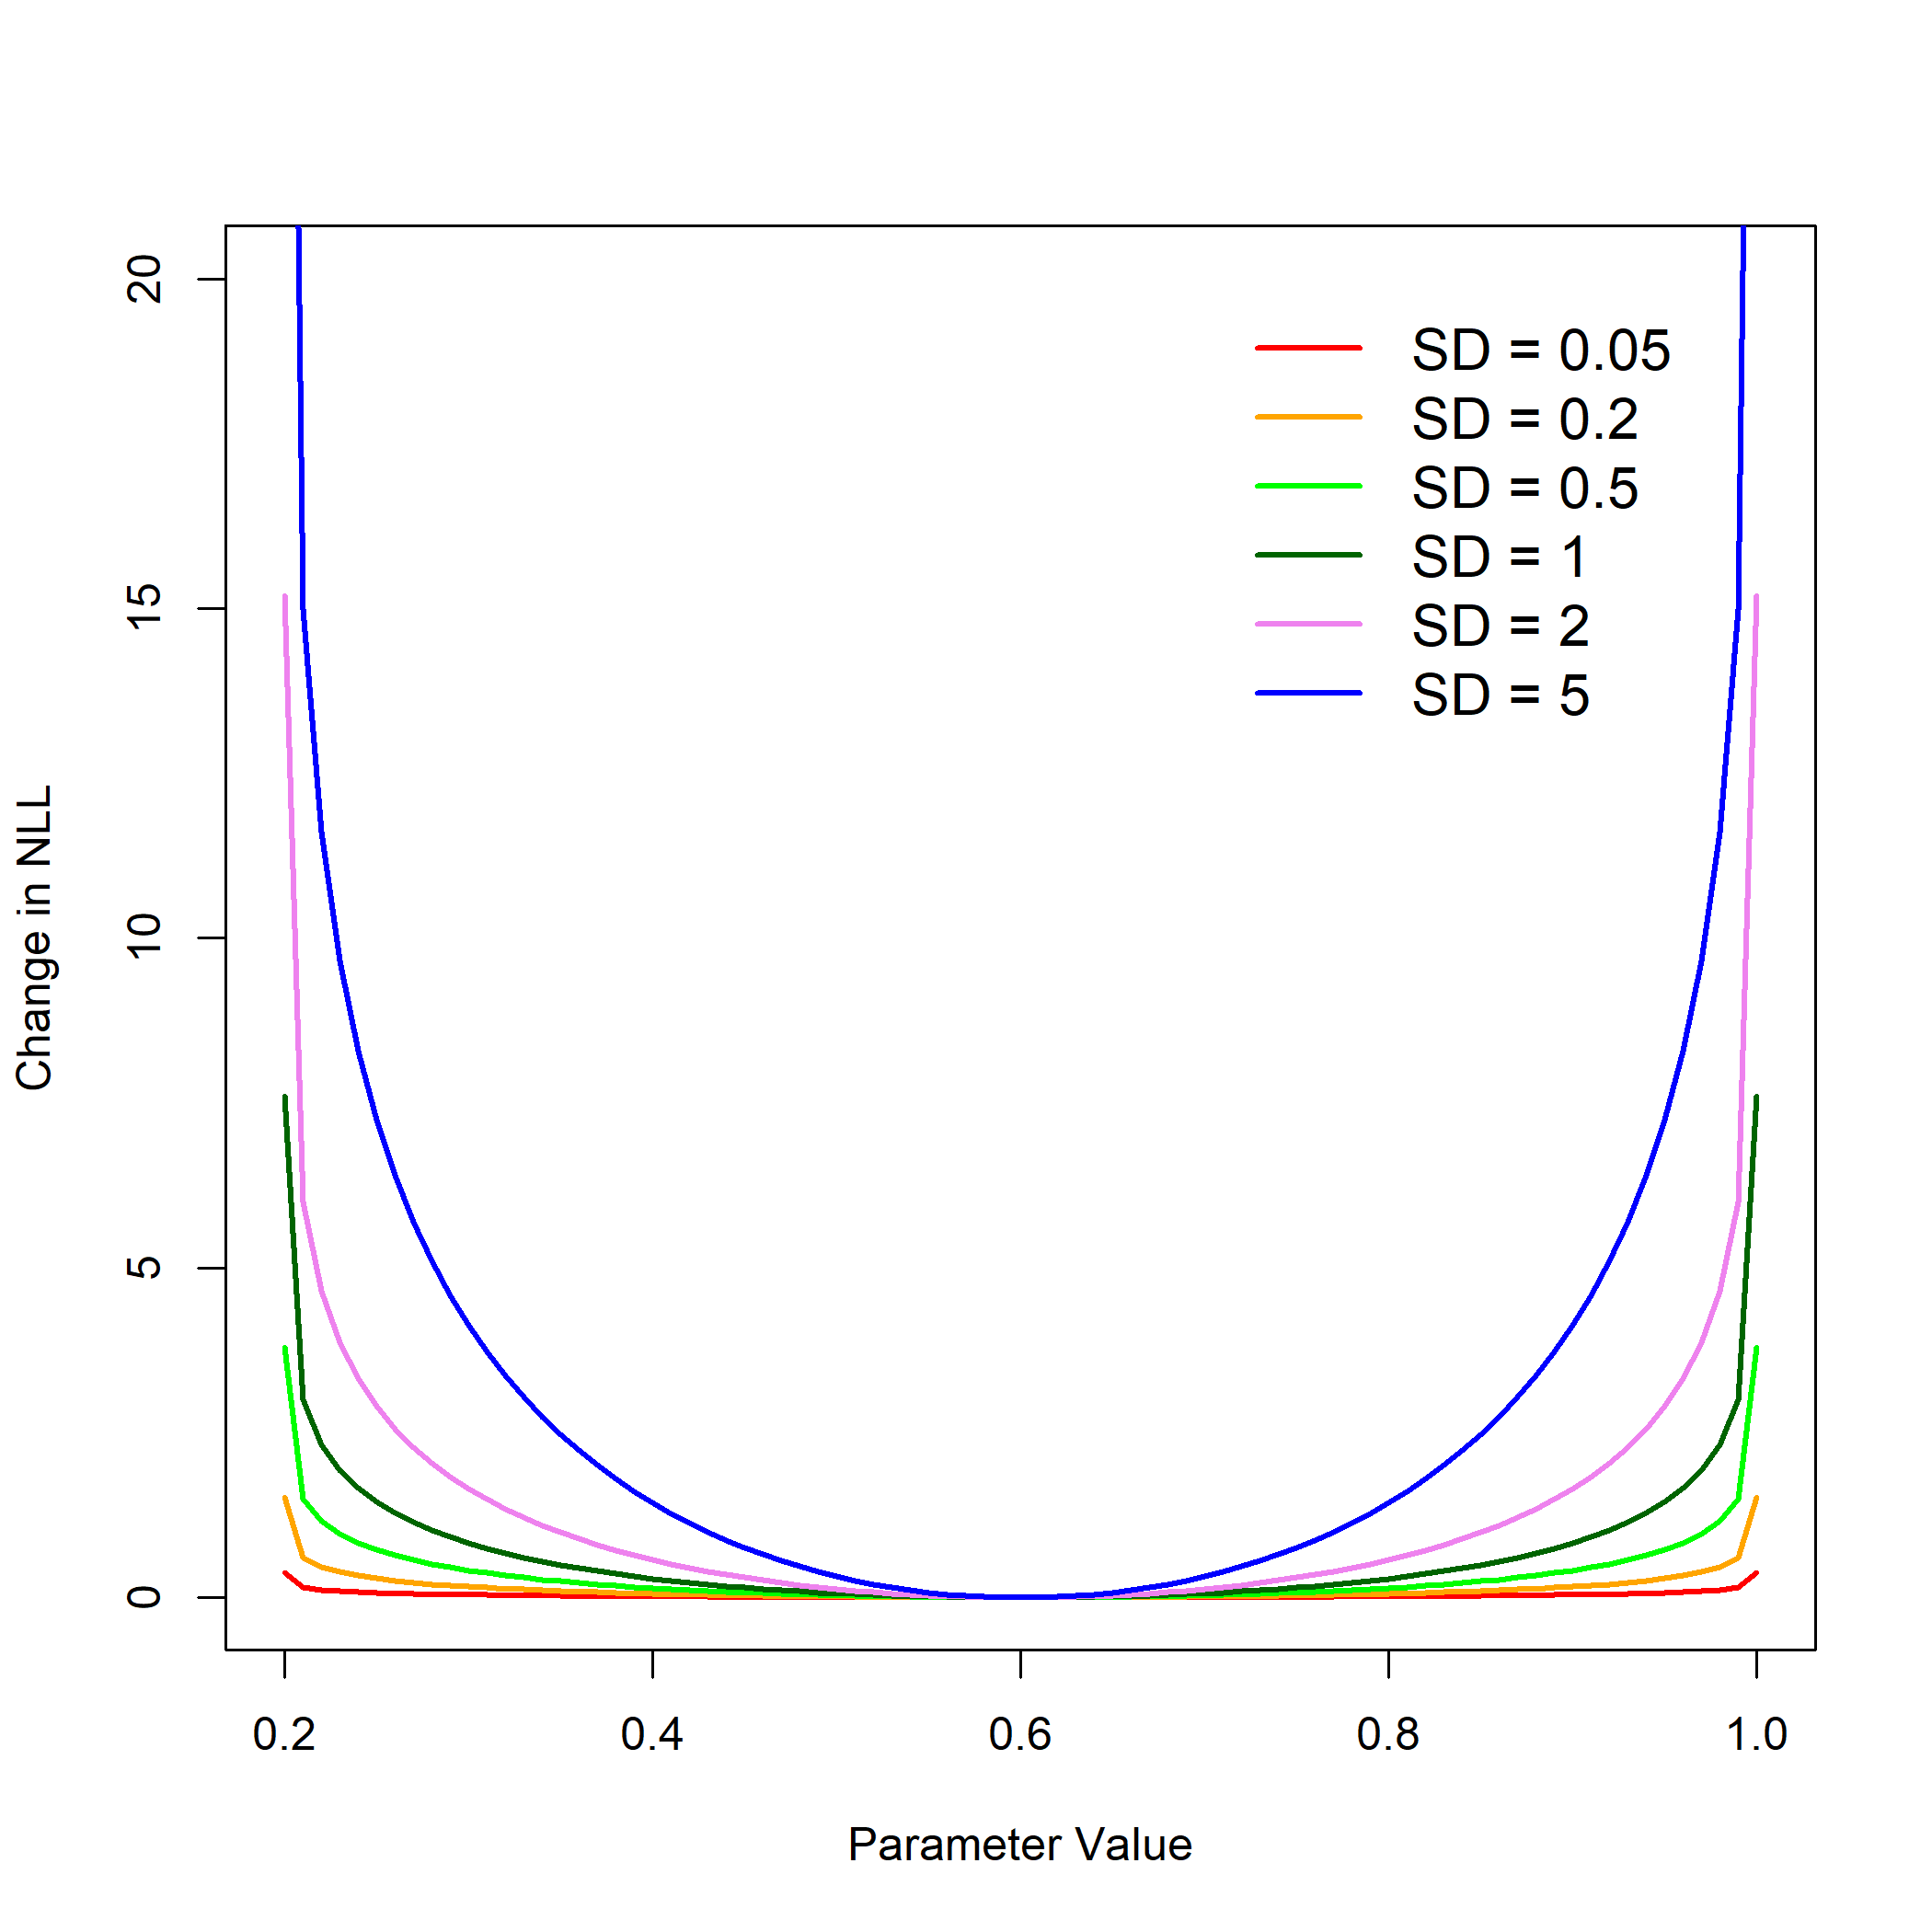
\includegraphics[scale = 0.6]{SymetricBeta}\\
	\end{center}
	\caption{Prior distributions for the symmetric beta distribution.}
	\end{figure}	

	
	\item \textbf{Prior Type = 2 = Beta prior}  \\ 
	The definition of $\mu$ is consistent with CASAL's formulation with the $Bprior$ and $Aprior$ corresponding to the $m$ and $n$ parameters.
	\begin{equation}
		\mu = \frac{Prior-P_{min}}{P_{max}-P_{min}} 
	\end{equation}
	\begin{equation}
		\tau  = \frac{(Prior-P_{min})(P_{max}-Prior)}{Pr\_SD^2}-1
	\end{equation}
	\begin{equation}
		Bprior  = \tau \cdot \mu
	\end{equation}
	\begin{equation}
		Aprior = \tau (1-\mu)
	\end{equation}
	
	\begin{equation}
		\begin{split}
			\text{Prior Likelihood} = & (1 - Bprior) \cdot ln(0.0001 + p - P_{min}) \\
			& + (1 - Aprior) \cdot ln(0.0001 + P_{max} - p) \\
			& - (1 - Bprior) \cdot ln(0.0001 + Prior - P_{min}) \\
			& - (1 - Aprior) \cdot ln(0.0001 + P_{max} - Prior)
		\end{split}
	\end{equation}

	\begin{figure}[h]
	\begin{center}
		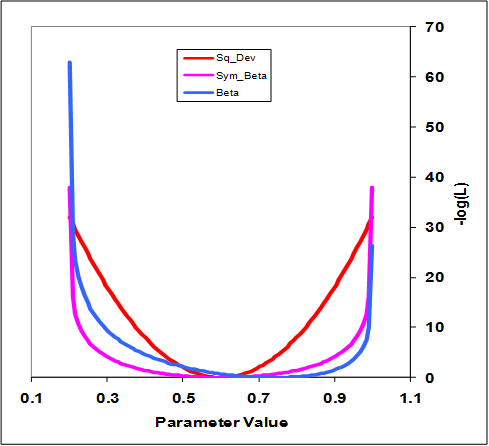
\includegraphics[scale = 0.9]{BetaComparison}\\
	\end{center}
	\caption{Comparison of the symmetric beta and the beta prior functions.}
	\end{figure}	

	
	\item \textbf{Prior Type 3 = Lognormal prior} \\ 
	Note that this is undefined for $p <= 0$ so the lower bound on the parameter must be > 0. The prior value is input into the parameter line in natural log space while the initial parameter value is defined in normal space (e.g. INIT = 0.20, PRIOR = -1.609438).
	\begin{equation}
		\text{Prior Likelihood} = \frac{1}{2} \left(\frac{ln(p)-Prior}{Pr\_SD}\right)^2
	\end{equation}
	
	\item \textbf{Prior Type 4 = Lognormal prior with bias correction} \\ 
	This option allows the prior mean value to be entered as the ln(mean). Note that this is undefined for $p <= 0$ so the lower bound on the parameter must be > 0.
	\begin{equation}
		\text{Prior Likelihood} = \frac{1}{2} \left(\frac{ln(p)-Prior + \frac{1}{2}{Pr\_SD}^2}{Pr\_SD}\right)^2
	\end{equation}
	
	\item \textbf{Prior Type 5 = Gamma prior} \\ 
	The lower bound should be 0 or greater.
	\begin{equation}
		scale = \frac{{Pr\_SD}^2}{Prior}
	\end{equation}
	\begin{equation}
		shape = \frac{Prior}{scale}
	\end{equation}
	\begin{equation}
		\text{Prior Likelihood} = -shape \cdot ln(scale) - ln\big(\Gamma(shape)\big) + (shape - 1) \cdot ln(p) - \frac{p}{scale}
	\end{equation}
	
	\item \textbf{Prior Type 6 = Normal prior} \\ 
	Note that this function is independent of the parameter bounds.
	\begin{equation}
		\text{Prior Likelihood} = \frac{1}{2} \left(\frac{p - Prior}{Pr\_SD}\right)^2
	\end{equation}
\end{itemize}

%=========Data Weighting
\hypertarget{appendB}{}
\subsection{Forecast Module: Benchmark and Forecasting Calculations}
\label{sec:forecast}

Stock Synthesis v.3.20 introduced substantial upgrades to the benchmark and forecast module. The general intent was to make the forecast outputs more consistent with the requirement to set catch limits that have a known probability of exceeding the overfishing limit. In addition, this upgrade addressed several inadequacies with the previous module, including:

\begin{itemize}
	\item The average selectivity and relative F was the same for the benchmark and the forecast calculations;
	\item The biology-at-age in endyr+1 was used as the biology for the benchmark, but biology-at-age propagated forward in the forecast if there was time-varying growth;
	\item The forecast module had a inefficient approach to calculation of overfishing limit (OFL) conditioned on previously catching ABC;
	\item The forecast module implementation of catch caps was incomplete and applied some caps on a seasonally, rather than the more logical annual basis;
	\item The Fmult scalar for fishing intensity presented a confusing concept for many users;
	\item No provision for specification of catch allocation among fleets;
	\item The forecast allowed for a blend of fixed input catches and catches calculated from target F; this is not optimal for calculation of the variance of F conditioned on a catch policy that sets annual catch limits (ACLs).
\end{itemize}

The v.3.20 module addressed these issues by:
\begin{itemize}
	\item Providing for unique specification of a range of years from which to calculate average selectivity for benchmark, average selectivity for forecast, relative F for benchmark, and relative F for forecast;
	\item Create a new specification for the range of years over which to average size-at-age and fecundity-at-age for the benchmark calculation. In a setup with time-varying growth, it may make sense to do this over the entire range of years in the time series. Note that some additional quantities still use their endyr values, notably the migration rates and the allocation of recruitments among areas. This will be addressed shortly;
	\item Create a multiple pass approach that rectifies the OFL calculation;
	\item Improve the specification of catch caps and implement specification of catch allocations so that there can be an annual cap for each fleet, an annual cap for each area, and an annual allocation among groups of fleets (e.g., all recreational fleets vs. all commercial fleets);
	\item Introduce capability to have implementation error in the forecast catch (single value applied to all fleets in all seasons of the year).
\end{itemize}

\myparagraph{Multiple Pass Forecast}
The most complicated aspect of the changes is with regard to the multiple pass aspect of the forecast.  This multiple pass approach is needed to calculate both OFL and ABC in a single model run. More importantly, the multiple passes are needed in order to mimic the actual sequence of assessment-management action - catch over a multi-year period. The first pass calculates OFL based on catching OFL each year, so presents the absolute maximum upper limit to catches. The second pass forecasts a catch based on a harvest policy, then applies catch caps and allocations, then updates the F's to match these catches. In the third pass, stochastic recruitment and catch implementation error are implemented and SS3 calculates the F that would be needed in order to catch the adjusted catch amount previously calculated in the second pass. With this approach, SS3 is able to produce improved estimates of the probability that F would exceed the overfishing F. In effect it is the complement of the P* approach. Rather than the P* approach that calculates the stream of annual catches that would have an annual probability of F>Flimit, SS3 calculates the expected time series of P* that would result from a specified harvest policy implemented as a buffer between Ftarget and Flimit.

The sequence of multiple forecast passes is as follows:
\begin{enumerate}
	\item Pass 1 (a.k.a. Fcast\_Loop1)
	\begin{enumerate}
		\item Loop Years
		\begin{enumerate}
			\item SubLoop (a.k.a. ABC\_Loop) = 1
			\begin{enumerate}
				\item R = f(SSB) with no deviations
				\item F = Flimit
				\item Fixed input catch amounts ignored
				\item No catch adjustments (caps and allocations)
				\item No implementation error
				\item Result: OFL conditioned on catching OFL each year
			\end{enumerate}
		\end{enumerate}
	\end{enumerate}
	\item Pass 2
	\begin{enumerate}
		\item Loop Years
		\begin{enumerate}
			\item SubLoop = 1
			\begin{enumerate}
				\item R = f(SSB) with no deviations
				\item F = Flimit
				\item Fixed input catch amounts ignored
				\item No catch adjustments (caps and allocations)
				\item No implementation error
				\item Result: OFL conditioned on catching ABC previous year. Stored in std\_vector.
			\end{enumerate}
			\item SubLoop = 2
			\begin{enumerate}
				\item R = f(SSB) with no deviations
				\item F = Ftarget to get catch for each fleet in each season
				\item Fixed input catch amounts replace catch from step 2
				\item Catch adjustments (caps and allocations) applied on annual basis (after looping through seasons and and areas within this year). These adjustments utilize the logistic joiner approach so the overall results remain completely differentiable.
				\item No implementation error
				\item Result: ABC as adjusted for caps and allocations
			\end{enumerate}
			\item SubLoop = 3
			\begin{enumerate}
				\item R = f(SSB) with no deviations
				\item Catches from Pass 2 multiplied by the random term for implementation error
				\item F = adjusted to match the catch*error while taking into account the random recruitments. This is most easily visualized in a MCMC context where the recruitment deviation and the implementation error deviations take on non-zero values in each instance. In MLE, because the forecast recruitments and implementation error are estimated parameters with variance, their variance still propagates to the derived quantities in the forecast.
				\item Result: Values for F, SSB, Recruitment, Catch are stored in std-vectors
				\begin{itemize}
					\item In addition, the ratios F/Flimit and SSB/SSBlimit or SSB/SSBtarget are also stored in std\_vectors.
					\item Estimated variance in these ratios allows calculation of annual probability that F > Flimit or B < Blimit. This is essentially the realized P* conditioned on the specified harvest policy.
				\end{itemize}
			\end{enumerate}
		\end{enumerate}
	\end{enumerate}
\end{enumerate}

\myparagraph{Example Effects on Correlations}
An example that illustrates the above process was conducted. The situation was a low M, late-maturing species, so changes are not dramatic. The example conducted a 10 year forecast and examined correlations with derived quantities in the last year of the forecast. This was done once with the full set of 3 passes as described above, and again with only 2 passes and stochastic recruitment occurring in pass 2, rather than 3. This alternative setup is more similar to forecasts done using previous model versions.

\begin{center}
	\begin{longtable}{p{0.4cm} p{2.75cm} p{3cm} p{1cm} p{0.4cm} p{2.75cm} p{2cm} p{1cm}}
		\hline
		 & \multicolumn{3}{l}{2 Forecast Passes with F from} & & \multicolumn{3}{l}{2 Forecast Passes with catch from} \\
		 & \multicolumn{3}{l}{ABC and random recruitment} & & \multicolumn{3}{l}{target F and equilibrium recruitment} \\
		\hline
		 & Factor X & Factor Y & Corr & & Factor X & Factor Y & Corr \\
		\hline
		A1 & F 2011 & RecrDev 2002 & -0.126 & A2 & F 2011 & RecrDev 2002 & 0.090 \\
		B1 & F 2011 & Recr 2002 & 0.312 & B2 & F 2011 & Recr 2002 & 0.518 \\
		C1 & ForeCatch 2011 & RecrDev 2002 & 0.000 & C2 & ForeCatch 2011 & RecrDev 2002 & 0.129 \\
		D1 & ForeCatch 2011 & Recr 2002 & 0.455 & D2 & Forecatch 2011 & Recr 2002 & 0.555 \\
		\hline		
	\end{longtable}
\end{center}

Correlation A2 shows a small positive correlation between the recruitment deviation in 2002 and the F in 2011. This is probably due to the fact that a positive deviation in recruitment in 2002 will reduce the chances that the biomass in 2011 will be below the inflection point in the control rule. This occurs because in calculating catch from F, the model effectively ``knows'' the future recruitments. I predict that this B1 correlation would be near zero if there was no inflection in the control rule.

Correlation A1 shows this turning into a negative correlation. This is because the future catches are first calculated from equilibrium recruitment, then when random recruitments are implemented, a positive recruitment deviation will cause a negative deviation in the F needed to catch that now ``fixed'' amount of future catch.

Correlations B1 and B2 are in terms of absolute recruitment, not recruitment deviation. Now overall model conditions that cause a higher absolute recruitment level will also result in a higher forecast level. No surprise there, and the correlation is stronger when variance is based on catch is calculated from F (B2).

Correlation C2 shows a positive correlation between recruitment deviation in 2002 and forecast catch in 2011. However, correlation C1 is 0.0 because the forecast catch in 2011 is set based on equilibrium recruitment and is not influenced by the recruitment deviations.

\myparagraph{Future Work}
\begin{itemize}
	\item More testing with high M, rapid turnover conditions
	\item Testing without inflection in control rule
	\item Consider separating implementation error into a pass \#4 so results will more clearly show effect of assessment uncertainty separate from implementation uncertainty
	\item Consider adding a random ``assessment'' error which essentially is a random variable that scales population abundance before passing into the forecast stage. Complication is figuring out how to link it to the correlated error in the benchmark quantities
	\item Because all of these calculations occur only in the standard deviation phase (sdphase) or the MCMC evaluation (mceval) phase, it would be feasible for mceval calls to add an additional pass that is implemented many times and in which random forecast recruitment draws are made.
	\item Factors like selectivity and fleet relative F levels are calculated as an average of these values during the time series. This is internally consistent if these factors do not vary during the time series (although clearly this is a stiff model that will underestimate process variance. However, if these factors do vary over time, then the average used for the forecast will under-represent the variance. A better approach would be to set up the parameters of selectivity as a random process that extends throughout the forecast period, and to update estimated selectivity in each year of the forecast based upon the random realization of these parameters.
\end{itemize}

	




\pagebreak

\section{Unique SS Configuration Advise}

\subsection{Continuous seasonal recruitment}
It is awkward in SS to set up a seasonal model such that recruitment can occur with similar and independent probability in any season of any year.  Consequently, some users have attempted to setup SS so that each quarter appears as a year.  They have set up all the data and parameters to treat quarters as if they were years (i.e., each still has a duration of 1.0 time step).  This can work, but requires that all rate parameters be re-scaled to be correct for the quarters being treated as years.

Another option is available.  If there is one season per year and the season duration is set to 3 (rather than the normal 12), then the season duration is calculated to be 3/12 or 0.25. This means that the rate parameters can stay in their normal per year scaling and this shorter season duration makes the necessary adjustments internally. Some other adjustments to make when doing quarters as years include:

\begin{itemize}
	\item Re-index all "year seas" inputs to be in terms of quarter-year because all are now season 1; increase end year (endyr) value in sync with this.
	\item Increase max age because age is now in quarters.
	\item In the age error definitions, increase the number of entries in accord with new max age
	\item In the age error definitions, recode so that each quarter-age gets assigned to the correct age bin. This is because the age data are still in terms of age bins; i.e., the first 4 entries for quarter-ages 1 through 4 will all be assigned to age bin 1.5; the next four to age bin 2.5;  you cannot accomplish the same result by editing the age bin values because the standard deviation of ageing error is in terms of age bin.
	\item In the control file, multiple the natural mortality age breakpoints and growth Amin and Amax values by 1/season duration.
	\item Decrease the R0 parameter starting value because it is now the average number of recruitments per quarter year.
	\item Edit the recruitment deviation (rec\_dev) start and end years to be in terms of quarter year.
	\item Edit any age selectivity parameters that refer to age to now refer to quarter age.
	\item If there needs to be some degree of seasonality to recruitment or some parameter, then you could create a cyclic pattern in the environmental input and make recruitment or some other parameter a function of this cyclic pattern.
\end{itemize}
	
A good test showing comparability of the 3 approaches to setting up a quarterly model should be done.

\pagebreak